% intro to chapter

	The subject of this thesis is inspired by a real scheduling problem as experienced by the NedTrain company.\footnote{http://www.nedtrain.nl}
	After a general introduction to the NedTrain company, we identify two main problems in scheduling for maintenance 
	engineering which according to our view are not only problems this particular company is facing, 
	but also are of general interest for the research field of scheduling.
	After a description of these research problems, 
	in subsequent chapters we derive some scientific research questions from these research problems and analyse them in full detail.  

\section{NS Group and NedTrain}

	% NS Group and its different parts
		NedTrain is a subsidiary company of Nederlandse Spoorwegen (NS) Group\footnote{http://www.ns.nl}, 
		the principal Dutch railway operator, 
		the origins of which can be traced back to the begining of the 19-th century.
		NS, which in 2016 made close to 90\% of their revenue from passenger trasport,
		serves approximately 1 million passengers per day mainly in the Netherlands but also in Germany, 
		the United Kingdom (UK) and other parts of Europe \cite{NS2016}. 
		Figure~\ref{fig-ns} shows the group of companies composing NS: 
		NS~Reizigers (or NSR, with approximately 11,000 staff), NedTrain (3,000), 
		NS~Stations (5,000, including retail) and Abellio (13,000).

		\begin{figure}
			\centering
			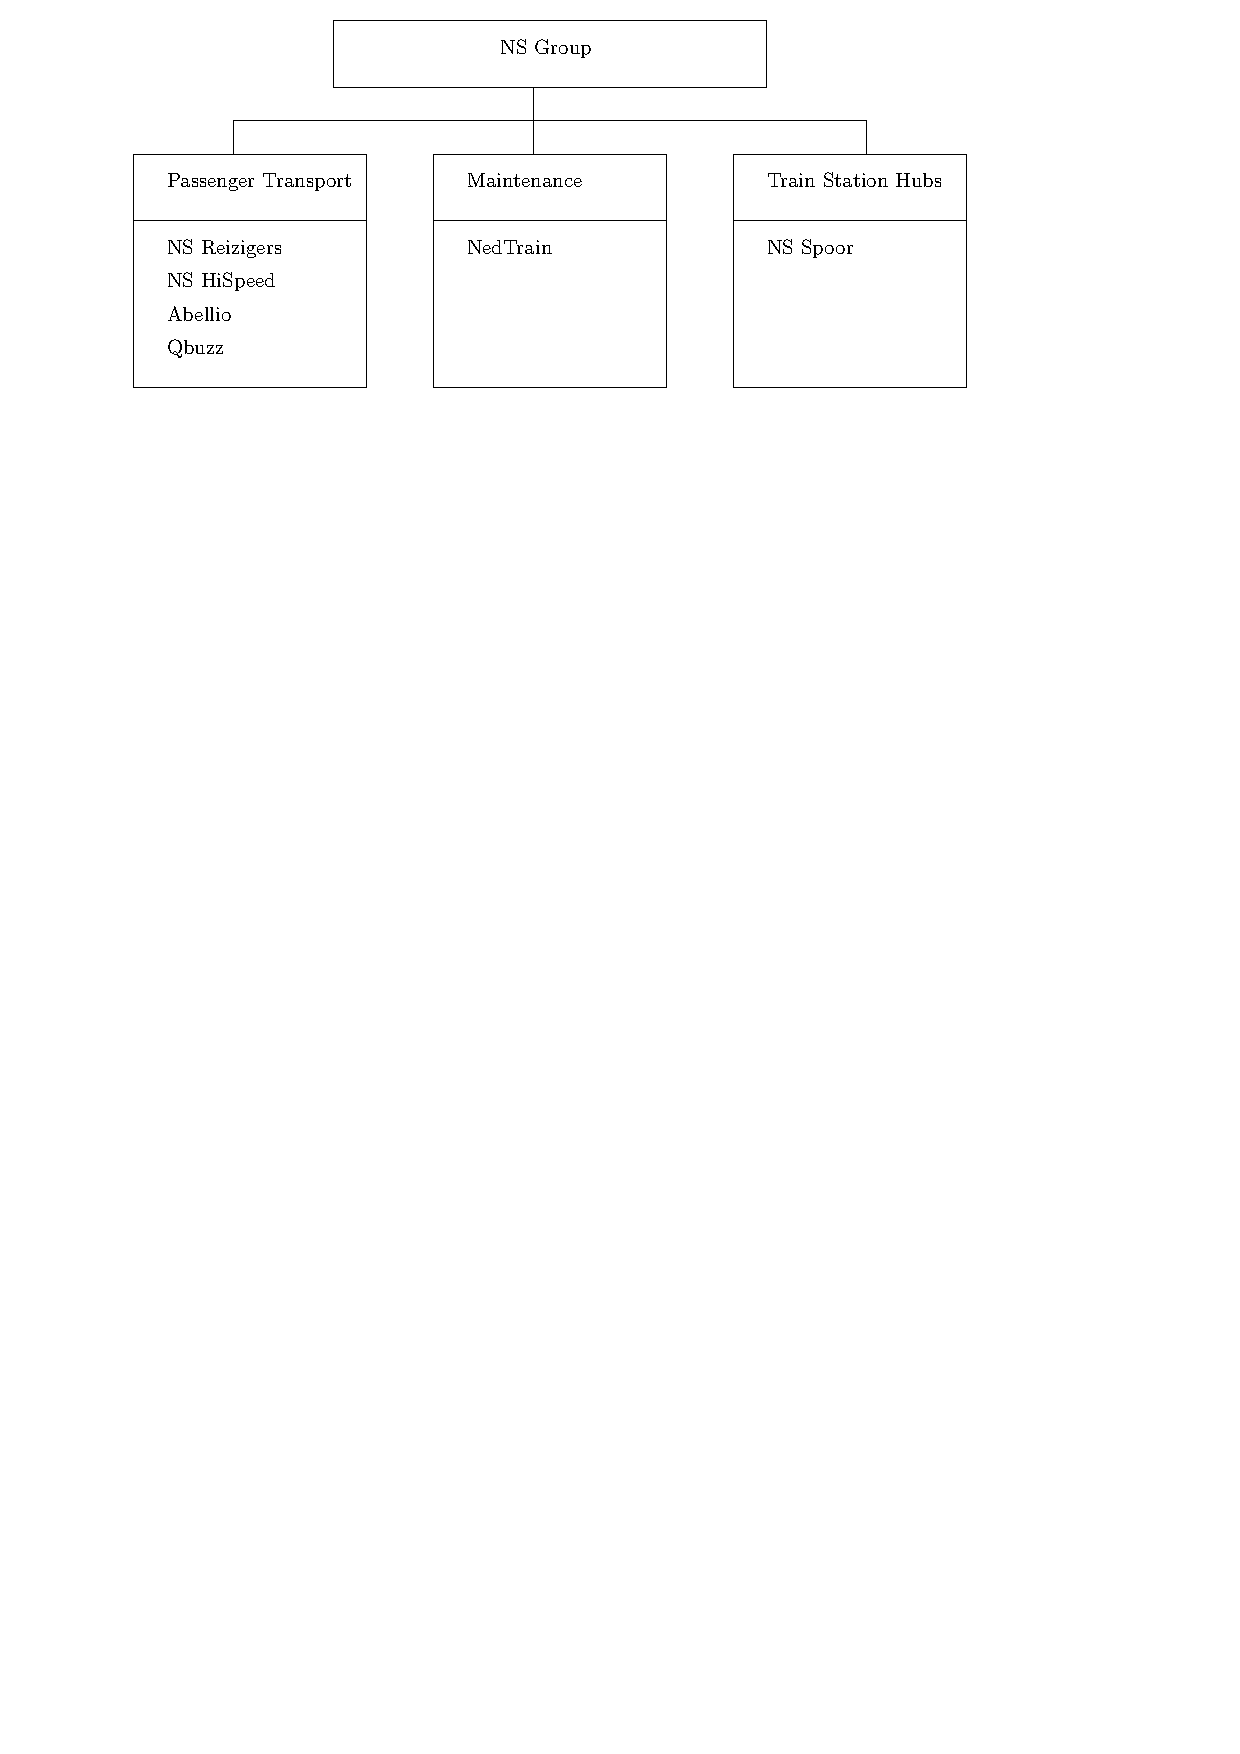
\includegraphics[width=0.95\textwidth]{chapter/introduction/ns-structure}
			\caption{NS Group and subsidiary companies (adapted from \cite{NS2016}).} 
			\label{fig-ns}
		\end{figure}

		% about NS Reizigers and NS Highspeed
		NS Reizigers and NS International operate the majority of trains on the Dutch rail network.
		They handle domestic and international passenger transportation, respectively,
		with a fleet of approximately 3000 rolling-stock units.
		Abelio handles passenger transportation in the UK and in Germany.
		% about NS stations
		NS Stations handles the development and operation of 410 large and small train stations,
		in cooperation with ProRail which is the company managing the Dutch rail network (not part of NS Group).

	% NedTrain; first-line service, technical maintenance and refurbishment
		NedTrain is responsible for maintaining a high availability rate for NS Reizigers and NS International trains, 
		providing the following types of maintenace: 
		\begin{description}
			\item[First-line service] 
			First-line service involves a daily cleaning and fixing of small technical problems 
			of each train at least once a day at one of thirty `servicebedrijf' (SB) facilities throughout the country. 

			\item[Technical maintenance]
			Once every three months or after a critical part has reached a certain mileage 
			each train goes to one of four NedTrain workshops, or `onderhoudsbedrijf' (OB) facilities for technical maintenance. 

			\item[Refurbishment] 
			Once or twice in its lifetime, a train might have to be refurbished to meet modern standards, 
			and refurbishment takes place in an overhaul and refurbishment workshop, in Haarlem.
		\end{description}
	% NedTrain: technical maintenance; the weekly schedule
		The work presented in this dissertation deals with scheduling problems 
		related to technical maintenance operations in a NedTrain workshop.
		NedTrain has four workshops for technical maintenance in The Netherlands: 
		in Amsterdam, Leidschendam, Onnen and Maastricht, and each location specializes in specific train types 
		(Figure~\ref{fig-workshop-1},\ref{fig-workshop-2}).
		Each workshop operates non-stop, 24 hours a day, covered by three 8-hour personnel shifts.
		For each workshop there is a week-long ``abstract'' schedule that mostly stays the same throughout the year.
		This schedule specifies when and which types of trains are expected to arrive at the workshop 
		and also when they must be returned for circulation in the rail network.
		This week-long abstract schedule is designed in harmony with the week-long time-tables used by NS Reizigers to carry passengers
		and such that NedTrain handles an evenly distributed workload over the year.

		Even though the abstract schedule stays more-or-less fixed throughout the year,
		the scheduling problem to be dealt with in a workshop changes on a weekly basis.
		This is because the list of necessary maintenance tasks for each specific train-fleet unit depends 
		on its past visits at the workshop and on its current condition.
		That is, each week the workshop operates based on an instantiation of the abstract schedule, 
		depending on the particular train units that will arrive for maintenance.
		In other words, the abstract schedule simply specifies arrival and due-dates for types of trains, 
		since from a passenger service point-of-view,
		it is only important that some train unit of a specific type is available when needed.

		About two weeks prior to an upcoming week, knowledge about which specific trains will arrive at the depot becomes available. 
		Each train is expected to arrive on a respective \emph{release-date} and 
		it must be delivered for circulation before a respective \emph{due-date}.
		If train constitutes a maintenance project then multiple projects will typically execute in parallel at the workshop.
		Depending on weather conditions and other factors, the number of trains under technical maintenance in 
		NedTrain workshops at the same time might peek to 300, i.e. to about 10\% of the entire fleet. 
		With about 50 tasks per train on average,
		up to 1500 tasks with uncertain durations might be taken into consideration when creating a weekly workshop schedule.
		
\section{NedTrain's Research \& Development program}

	NedTrain has the ambition to be a first class European rolling stock maintenance company. 
	To support their ambition, NedTrain intiated the `Rolling Stock Life-Cycle Logistics' (RSLCL) 
	applied research and development program, in cooperation with several Dutch universities.
	The main question to be addressed by the RSLCL program can be formulated as follows:
	\begin{quote}
		How to obtain and maintain the best combination of rolling stock, maintenance
		operations and supply chain, within the context of railway operations, to enable
		our customers to deliver competitive high quality services to their passengers? \cite{huisman2009}
	\end{quote}

	The search for an answer to this question is mostly directed by the following
	Key Performance Indicators (KPIs) concerning the train-fleet of NS:
	\begin{enumerate}
		\item total Cost of Ownership (or Life-Cycle Cost) of the fleet;
		\item availability of sufficient transport capacity;
		\item reliability of transport;
		\item quality of transport.
	\end{enumerate}
	
	The scope of the RSLCL program is too wide to be undertaken as a single study.
	As such, the program has been divided into three different levels:
	the strategic, tactical and operational level,
	each associated with a different time-scale of planning and control.
	In what follows we give a summary for each of the three levels of the program.
	
	\begin{description}
	\item[Strategic]
	Since rolling stock has several decades of life-time,
	decisions regarding the acquisition of rolling stock constitute long-lasting investments that tie up resources for years.
	Moreover, buying rolling stock amounts to less than 40\% of the overall life-cycle cost.
	That is, most money is spent on operation and maintenance during the years rolling stock is in service.
	Since this amount of money is mostly allocated during the acquisition process,		
	the main objective at the strategic level is the development of methods for
	ranking acquisition options from the perspective of \emph{supportability} and the design optimal logistics support.
	
	\item[Tactical]
	The tactical level concerns the allocation and planning of spare parts, 
	human resources and maintenance tasks and the management of physical flows,
	given that decisions about the acquisition of rolling stock 
	and the maintenance infrastructure have been made and will remain fixed on the intermediate timescale.
	Moreover, the tactical level considers the impact of changing the supply chain in order to
	outsource some of the maintenance operations to the manufacturer of rolling stock.
	
	\item[Operational]
	The operational level concerns the effective scheduling of maintenance operations in a NedTrain workshop,
	in order to ensure timely delivery of rolling stock for circulation in the rail network.
	Maintenance tasks having uncertain durations
	(partly because of the conditional nature of repairs, i.e. not knowing which repairs must be performed until
	after the arrival and inspection of a train in the workshop) makes the scheduling of technical maintenance a rather challenging feat.
	Due to the possibility of maintenance running late,
	ensuring a certain level of fleet availability relies on buffer stock.		
	The main objective at the operational level is to reduce the total cost of fleet ownership
	by improving the planning and scheduling process at the workshop,
	which in turn would allow the level of buffer stock to decrease.	
	\end{description}
	 
	In a joint cooperation with the technical universities in the Netherlands, 
	three research projects have been carried out:
	Research concerning the strategic level has been conducted by Parada Puig et al. \cite{parada:2015} at the University of Twente and
	research concerning the tactical level has been conducted by Arts et al. \cite{arts2013spare} at the Technical University of Eindhoven.
	Research concerning the operational level is undertaken by Wilson et al. \cite{wilson:2016} at the Technical University of Delft.
	As a follow-up to the work of Wilson et al., this dissertation also focuses on the operational level,
	i.e. the scheduling of maintenance tasks in a NedTrain workshop, in the face of uncertainty.		
	%
	% TODO: what michel achieved wrt scheduling
	% Here is a slight gap: you have to mention what the essential contribution is of Michel’s thesis and what he left open.
	% he did not pay attention to uncertainty
	%
	The overall research effort concerning all three levels of the program 
	is monitored and directed at regular Steering Group meetings
	that take place (up to) four times a year, involving a representative for each of the stakeholders.
	
	In what follows we focus on the current scheduling process at NedTrain
	and highlight the basic issues caused by the presence of uncertainty.
	Moreover, we propose two potential approaches for better dealing  with uncertainty
	and formulate corresponding research problems that we will be addressing in our work.

\section{Basic issues with maintenance scheduling}
	% workshop pictures
		\begin{figure}
			\centering
			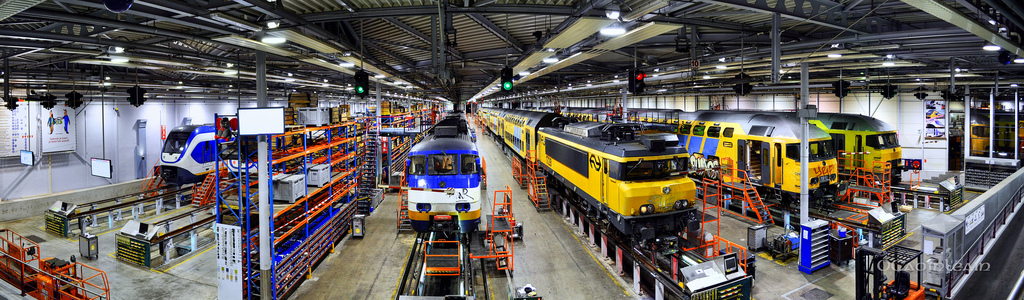
\includegraphics[width=0.9\textwidth]{chapter/introduction/workshop-1}
			\caption{Inside the Leidschendam workshop.}
			\label{fig-workshop-1}
		\end{figure}

		\begin{figure}
			\centering
			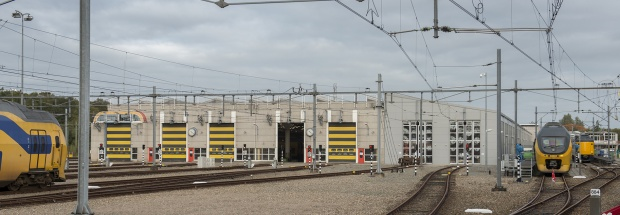
\includegraphics[width=0.9\textwidth]{chapter/introduction/workshop-3}
			\caption{Shunting yard of the workshop in Onnen.}
			\label{fig-workshop-2}
		\end{figure}

	% what is the complication
		As with most (if not all) real-life applications of scheduling,
		the main complication in NedTrain's case is that tasks have uncertain durations.
		In a maintenance workshop, dismounting parts is a very common operation.
		In contrast with assembling a part (as in production), the time needed for a dismount tends to vary according to uncontrollable factors.
		Another source of uncertainty is due to the conditional nature of repairs.
		That is, some tasks involve inspecting a certain part and then repairing it, if necessary.
		The duration of such tasks is by definition highly uncertain since whether 
		any time will be spent on repairing the part is unknown in advance.

		A schedule, on the other hand, is created subject to temporal and resource constraints and allocates a fixed amount of time per task.
		If the amount of time needed (i.e. the outcome duration) exceeds the amount of time allocated for a task (i.e. the predicted duration),
		then some other tasks might have to be rescheduled in order to comply with temporal constraints and/or resource constraints.
		As a result, scheduling in an uncertain environment is not so much about finding a good schedule 
		as it is about keeping the schedule up-to-date with outcome durations without deteriorating its quality in the long run.

	% what is done now
		Currently, the scheduling process at NedTrain is semi-automated.
		A baseline schedule is created and adapted during task execution as necessary by a team of 
		planners who rely on their domain expertise and the help of software like ProPlan or Microsoft Excel.
		To cope with uncertainty, a significant amount of slack is inserted in the schedule.
		Moreover, as a last resort option, some tasks might be skipped and postponed for the next workshop visit in order to deliver a train on time.

	% the difficulty of slack insertion
		Adding too much slack stabilizes dispatching times (meaning they will probably not change much during task execution) 
		but at the same time it compromises efficiency or punctuality, because the schedule becomes long.
		Adding too little slack, on the other hand, means we will have to update the schedule often during execution.
		Aggressive and frequent rescheduling of human resources is highly undesirable as it creates confusion, or nervousness, 
		which in the end also hinders performance.
	
	% how to improve the current approach
		In the NedTrain workshop we are dealing with large scheduling problems 
		with several hundreds of tasks and constraints and a great deal of uncertainty.
		The demand to keep the schedule up-to-date with a changing environment without introducing confusion, 
		or ``shop-floor nervousness'' while achieving a high degree of timeliness,
		might easily outstrip the capacity of human planners.
		The current approach works but there is clearly room for improvement, as we see more in detail in the next section.
		The mission of NedTrain's R\&D, at the operational level, 
		is to modernize the scheduling process by finding state-of-the-art scheduling techniques 
		that can be adapted and/or extended for the particular requirements of the NedTrain workshop.
		Based on eventual research findings, the purpose is to develop custom-tailored scheduling tools that can help 
		operational planners to enhance punctuality and eliminate nervousness at the workshop, without sacrificing throughput.

	% repair picture
		\begin{figure}
			\centering
			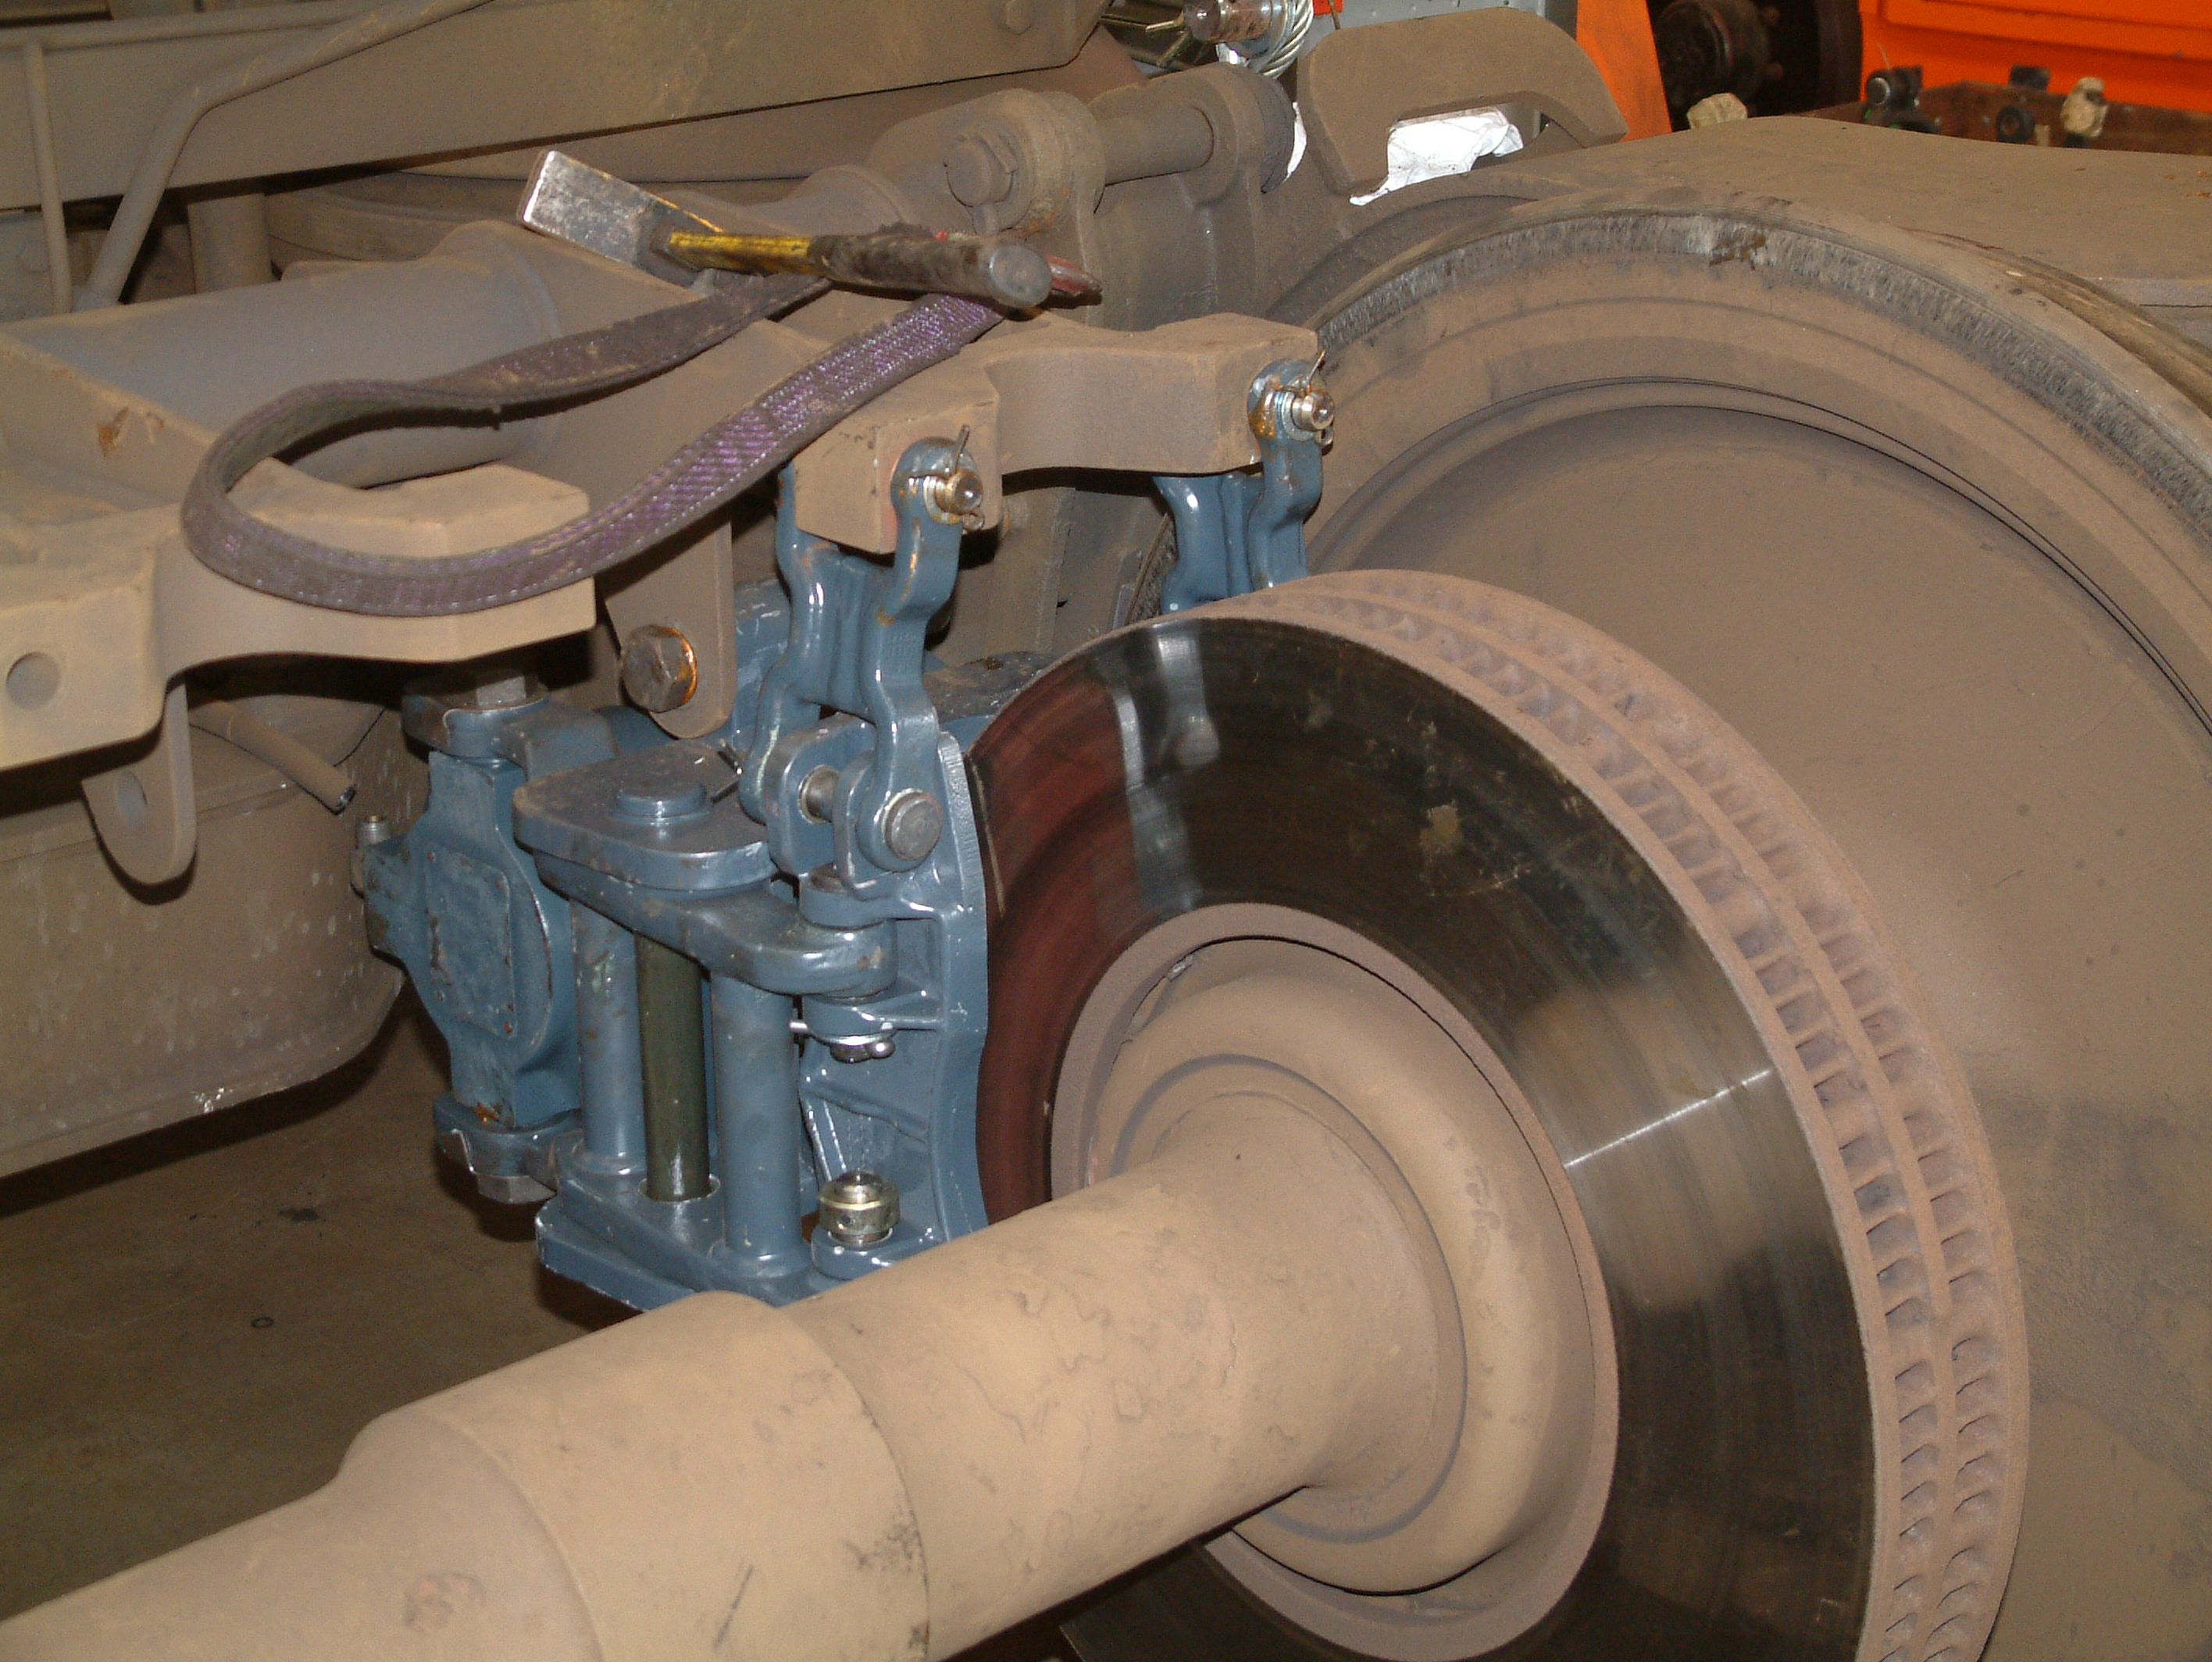
\includegraphics[height=0.3\textheight]{chapter/introduction/workshop-4}
			\caption{Replacement of a faulty part.}
			\label{fig-workshop-4}
		\end{figure}

\section{Research Problems}
\label{chapter:introduction:research-problems}

	% the two options of management
		Since human resources are very much against the idea of being rescheduled frequently,
		management has to choose between two options: 
		\begin{enumerate}[(I)]
			\item Adding sufficient slack to avoid the need for continuous rescheduling (nervous process), or
			\item give human resources the autonomy to take the decisions to (re)schedule themselves.
		\end{enumerate}
		In other words, unless management is able to provide a schedule that remains stable (i.e. relatively unchanged) during execution,
		people would rather have the freedom to (re)schedule themselves and stay in control.

	% what it means to pursue option 2
		Pursuing option two (letting people reschedule themselves and be in control) involves transitioning from regular schedules, 
		padded with slack, to \emph{flexible schedules}.
		Instead of specific dispatching times, 
		a flexible schedule prescribes a space of potential schedules, 
		from which people can pick suitable dispatching times on-the-fly.

	% the challenges involved 
		The main difficulty with letting people choose their own dispatching times is ensuring that scheduling constraints will be satisfied,
		i.e. the realization of a feasible schedule.
		Human resources in the NedTrain workshop are organized in groups, or work-teams. 
		Each team is led by a corresponding foreman and is responsible for the completion of a certain subset of tasks.
		Moreover, each team would like to be able to plan-ahead and operate as an independent unit.
		Tasks belonging to different teams are usually interrelated, however,
		because of having to share workshop resources and satisfy certain temporal constraints between tasks.

		Ensuring the generation of a schedule satisfying workshop constraints 
		should not rely on synchronous communication between teams;
		it is important that teams retain their independence.
		That is, teams should not be expected to negotiate with other teams over the dispatching of hundreds of tasks.
		This would certainly compromise performance and create confusion.
		The main challenge in developing such a flexible scheduling technique, then, 
		is ensuring constraint satisfaction by dispatching decisions taken in isolation.
		To make this possible, a flexible schedule should provide appropriate 
		boundaries within which individual teams can make decisions, 
		while offering as much flexibility as possible.
		In pursuit of such scheduling techniques, 
		the first part of this thesis is devoted to addressing the following problem:

		\begin{quote}
			\textbf{Research Problem I.}\\
			\emph{How to compute flexible schedules for independent work-teams that can be easily adapted to changes in the environment?}
		\end{quote}

	% what it means to pursue option 1
		Having discussed the potential of pursuing option two,
		we will now also consider the potential to pursue the more traditional first option, 
		i.e. using regular schedules with sufficient slack to avoid continuous rescheduling.
		In line with existing literature,
		we shall base our discussion on the concepts of stability and robustness. 
		Stability refers to the quality to preserve dispatching times relatively unchanged during task execution.
		Robustness, on the other hand, guarantees good performance or timeliness 
		with respect to the given due-dates (and does not imply stability). 

	% the challenges involved 
		Determining at which points in the schedule and at what quantities should slack be inserted 
		in order to strike a good balance between stability and robustness can be difficult,
		because of the intricate manner in which uncertainty accumulates in a schedule.
		For example, more slack is needed near the end of a schedule since
		tasks that start later are susceptible to the accumulated effects of uncertainty,
		in contrast with tasks that started earlier.
		Moreover, more slack is necessary in order to protect the 
		dispatching time of a task with many temporal dependencies, and so on.
		In pursuit of a sophisticated and fully automated method for inserting slack,
		we are interested in dealing with the following problem:

		\begin{quote}
			\textbf{Research Problem II.}\\
			\emph{How to compute robust and stable schedules for work-teams in order to deal with uncertainty in the duration of maintenance tasks?}
		\end{quote}

		We then considered two potential methods for dealing with uncertainty in task durations and formulated two corresponding Research Problems.
		Addressing these problems, which we feel might be of interest to other organizations besides NedTrain,
		is precisely the purpose of our research.
		The next section outlines the structure of the dissertation, 
		which consists of Part I and Part II, 
		each devoted to the corresponding Research Problem.

\section{Organization of the thesis}
	% split in two parts: differences and a common theme
		Our research findings concerning the two approaches for dealing with uncertainty discussed earlier are presented, 
		respectively, in Part I and Part II.
		%Both approaches belong to the general research area of scheduling under uncertainty, 
		%but uncertainty has a different meaning in each of the two cases.
		Despite their differences, Part I and Part II have an underlying theme in common: 
		beyond finding a fixed schedule for a given scheduling problem,
		we are interested in finding a strategy for adjusting, or generating the schedule, 
		in a continuous scheduling process.

	% Part I 
		Part I (Chapters~2,3,4) focuses on the approach
		of letting people (re)schedule themselves in the workshop.
		To enable this approach from a technical standpoint, 
		we turn to the research area concerning Simple Temporal Porblem (STP) constraints.
		Such constraints restrict the minimum and maximum temporal distance between the dispatching of pairs of events.
		It is assumed that each event is associated with a respective actor that will choose when to dispatch his event from a respective time interval,
		in a non-deterministic manner.
		%Uncertainty in this case results from not being able to predict how the actor will choose within the given interval.
		We are interested in finding a \emph{flexible} strategy for initializing these time intervals and keeping them up-to-date as choices are being made,
		striving to maximize the freedom (or flexibility) with which actors can make choices.
		At the same time, we are also guaranteeing the formation of a feasible schedule
		regardless of the non-determinism with which actors choose within those intervals.
		%
		Chapter~2 summarizes important concepts from the research area of STPs.
		Emphasis is put on the work of Wilson et al. \cite{wilson:2016},
		in which the use of STPs for the NedTrain workshop was originally examined, 
		and whose findings we extend in this thesis.
		Following the summary of important concepts, 
		we view Research Problem I through the prism of STP-related scheduling frameworks 
		and break it down into more specific Research Questions I.1, I.2, and I.3.
		Chapters 3 and 4 present our research findings for answering these questions, 
		effectively addressing Resarch Problem I at a technical level.
	
	% Part II
		Part II (Chapters~5,6,7) focuses on generating a schedule with sufficient slack to absorb the effects of uncertainty,
		prescribing a stable dispatching time for each task.
		To enable this approach from a technical standpoint we turn to the research area of Stochastic Task Networks,
		i.e. networks of precedence constraints between pairs of tasks with random durations.
		This second approach involves utilizing information from previous maintenance sessions 
		in order to model the uncertain duration of each task as a random variable with a known probability distribution.
		We are interested in finding a dispatching strategy that enables us to predict with some confidence the outcome start-times of the tasks, 
		even though the outcome task durations are unpredictable.
		More in particular, we are interested in finding a strategy that optimizes the trade-off between two conflicting qualities:
		dispatching tasks efficiently and dispatching tasks predictably.
		%
		Chapter~3 summarizes important concepts and problems from the area of stochastic scheduling;
		mostly focusing on precedence constraint networks between tasks with random durations.
		Through a stochastic scheduling point-of-view,
		we break-down Research Problem II into specific Research Questions II.1 and II.2.
		Following, Chapters 6 and 7 present our research findings when attempting to answer those questions.

	% Part III
		Part III concludes the dissertation.
		In Chapter~8 we revisit the research questions formulated in Chapter~2 and Chapter~5 and assess whether we managed to find adequate answers.
		Then we do the same from a more high-level standpoint for the research problems formulated earlier in this chapter.
		Finally, we present a collection of interesting problems that could be addressed in future work.

